\documentclass[12pt,thmsa]{article}
\usepackage{natbib}
\usepackage{amsfonts}
\usepackage{amssymb}
\usepackage[pdftex]{graphicx}
\usepackage{algorithm}
\usepackage[noend]{algpseudocode}

\newcommand{\subjectto}{\mathrm{subject\ to:}}
\newcommand{\minimize}{\mathrm{minimize}}

\newtheorem{complexity}{Complexity}
\newtheorem{theorem}{Theorem}
\newtheorem{lemma}{Lemma}
\newtheorem{definition}{Definition}
\def\qed{\hfill \quad \vrule height4.17pt width4.17pt depth0pt} 
\newenvironment{proof}[1][Proof]{\noindent \textbf{#1:} }{\qed}
\newcommand{\maxflow}{\mathrm{maxflow(}n,m\mathrm{)}}
\newcommand{\ixtet}{I{\scriptsize X}T{\scriptsize E}T\hspace*{1mm}}
\def\subsetnoteq{\subsetneq}

\begin{document}

\thispagestyle{empty}

\begin{center} 
{\sc ILOG\ Technical report number 05-002}

{\sc \copyright\ ILOG\ 2005 all rights reserved}
\end{center} 

\hrulefill
\vspace{6cm}

\begin{center}
{\Large {\bf Randomized Large Neighborhood Search for Cumulative Scheduling}} \\
\vspace{1.5cm}
{\large Daniel Godard, Philippe Laborie, Wim Nuijten} \\
\vspace{0.7cm}

ILOG\ Gentilly \\
9, rue de Verdun \\
94253 Gentilly

\end{center}
\newpage

\begin{abstract}
\begin{quote}

This technical report presents a Large Neighborhood Search (LNS) approach based
on constraint programming to solve cumulative scheduling problems. It
extends earlier work on constraint-based randomized LNS for
disjunctive scheduling as reported in \cite{NuijtenLePape98}. A
breakthrough development in generalizing that approach toward
cumulative scheduling lies in the presented way of calculating a
partial-order schedule from a fixed start time schedule. The approach
is applied and tested on the Cumulative Job Shop Scheduling Problem
(CJSSP). An empirical performance analysis is performed using a
well-known set of benchmark instances. The described approach obtains
the best known performance reported to date on the CJSSP. It not only
finds better solutions than ever reported before for 33 out of 36 open
instances, it also proves to be very robust on the complete set
of test instances. Furthermore, among these 36 open instances, one is now 
closed. As the approach is generic, it can be applied to
other types of scheduling problems, for example problems including
resource types like reservoirs and state resources, and objectives
like earliness/tardiness costs and resource allocation costs.

\end{quote}
\end{abstract}


\section{Introduction}

Scheduling can be described as the process of allocating scarce
resources to activities over time. Traditionally, the class of {\em
disjunctive} scheduling problems, where each resource can execute at
most one activity at a time, has received a lot of attention. In this
paper we are concerned with the class of {\em cumulative} scheduling
problems, where resources may execute several activities in parallel,
provided the resource capacity is not exceeded.

Many practical scheduling problems are cumulative scheduling problems
and in recent years the attention for cumulative scheduling problems
in general \cite{BaptisteLePape99} and the resolution of these
problems by way of local search in particular has increased
\cite{Cesta2000,Michel2003,Palpant2004}. Our approach is an
implementation of the Large Neighborhood Search framework
\cite{Shaw1998} which is based upon a process of continual relaxation
and re-optimization. We apply this approach on a generalization of the
Job Shop Scheduling Problem \cite{French82} which we call the
Cumulative Job Shop Scheduling Problem (CJSSP). Informally, this
problem can be stated as follows. Given are a set of {\em jobs} and a
set of {\em resources}. Each job consists of a set of {\em activities}
that must be processed in a given order.  Furthermore, for each activity
is given an integer {\em processing time}, a resource by which it has
to be processed, and an integer {\em demand} that represents the amount 
of resource required by the activity. Once an activity is started, it is
processed without interruption. Resources may process several
activities simultaneously. To this end, for each resource is given an
integer {\em capacity}. A resource can simultaneously process only
those sets of activities whose total demand do not exceed the
capacity of the resource. A {\em schedule} assigns a start time to
each activity. A {\em feasible} schedule is a schedule that meets the
order in which the activities must be processed and in which the
capacity of none of the resources is exceeded at any point in
time. One is asked to find an {\em optimal} schedule, i.e, a feasible
schedule that minimizes the {\em makespan} of the schedule, the
makespan being defined as the maximum completion time of any of the
activities. We remark that the CJSSP is the optimization variant of
the Multiple Capacitated Job Shop Scheduling Problem of
\cite{Nuijten94,NuijtenAarts96}.

The organization of the remainder of the paper is as follows. First we
define the CJSSP after which we present the LNS approach we
propose. We then present the computational results to finally discuss
the conclusions of the paper and potential directions of future
research.


\section{The Cumulative Job Shop Scheduling Problem}\label{SCJSSP}

\newcommand{\calA}{{\cal A}}
\newcommand{\calJ}{{\cal J}}
\newcommand{\calR}{{\cal R}}
\newcommand{\dZ}{{\sf Z\hspace*{-0.44em}Z}}

The Cumulative Job Shop Scheduling Problem (CJSSP) can be formalized
as follows. We are given a set $\calA$ of activities, a set $\calR$ of
resources, and a set $\calJ$ of jobs, each job $j$ consisting of a
sequence of activities $(a_{1},...,a_{n})$. Each activity $a \in
\calA$ has a processing time $pt(a)$ and a demand $d(a)$
for resource $r(a)$ to be executed. Each resource $r \in \calR$ has a
capacity $C(r)$ and a binary relation $\prec$ is
given that decomposes $\calA$ into chains, such that every chain
corresponds to a job. A {\em schedule} is an assignment $s: \calA
\rightarrow \dZ^+_0$ assigning a positive start time $s(a)$ to each
activity $a \in \calA$. A schedule $s$ is {\em feasible} if it
satisfies the {\em precedence constraints} between
each pair of consecutive activities in a job:
\begin{eqnarray}
	\forall_{a,a' \in \calA \mid a \prec a'} \: s(a) + pt(a) \leq s(a')
	\label{precedence}
\end{eqnarray}\\
and the {\em resource capacity constraints} for each resource:
\begin{eqnarray}
	\forall_{r \in \calR} \: \forall_{t \in \dZ^+_0}
	\sum_{a \in \calA_{r} \mid s(a) \leq t < s(a)+ pt(a)} \: d(a) \leq C(r)
	\label{resourecapacity}
\end{eqnarray}
where $\calA_{r} = \{a \in \calA \mid r(a) = r\}$. One is asked to
find an {\em optimal schedule} which is a feasible schedule that
minimizes the {\em makespan} defined as $\max_{a \in \calA}
s(a)+pt(a)$.


\section{Randomized Large Neighborhood Search} \label{SProblemSolving}

Our approach is an implementation of the Large Neighborhood Search
(LNS) framework \cite{Shaw1998} which is based upon a process of
continual relaxation and re-optimization. It is a generalization of
the randomized LNS approach for the Job Shop Scheduling Problem of
\cite{NuijtenLePape98}. The LNS framework is illustrated in
Figure~\ref{fig:approach}. A first solution is computed and
iteratively improved. Each iteration consists of a relaxation step
followed by a re-optimization of the relaxed solution. This process
continues until some condition is satisfied (for instance a time limit
or a number of non-improving iterations).

\begin{figure}[h]
	\centering
		\includegraphics[width=7cm]{figures/approach2.pdf}
	\caption{LNS Framework}
	\label{fig:approach}
\end{figure}

One of the first approaches that used LNS was on the Job Shop
Scheduling Problem \cite{ApplegateCook91}. One of the challenges for
applying LNS to cumulative scheduling (and to even more complex
scheduling problems in general) is that most of the available
algorithms to solve cumulative scheduling problems produce solutions
with fixed start times. In this context, relaxing a solution by only
unfreezing the start time of some activities in the schedule provides
limited flexibility to re-optimize the relaxed solution. Previous work
on cumulative job shop problems \cite{Cesta2000,Michel2003} avoids
this issue by generating precedence constraints as decisions and producing
a temporal constraint network which is more flexible thus more adequate 
for LNS than a completely instantiated schedule. ~\cite{Palpant2004} also applied an LNS
framework on resource-constrained project scheduling problems. They avoid the issue of lack of flexibility by
composing a solution method to solve the sub-problem which does not
necessarily decrease the makespan with a forward/backward heuristic
\cite{Li1992} to left-shift frozen activities so as to take advantage
of the more compact solution with relaxed activities.

In this paper, we investigate a slightly different approach where any
algorithm can be used to produce a first solution and to iteratively
re-optimize the current solution. The main advantage of this approach
is its genericity, i.e., the type of search algorithm used to compute first
solutions or for re-optimization is completely orthogonal to the type
of LNS relaxation that is used. Consequently one can for instance
apply this approach to problems involving minimization of
earliness/tardiness costs or resource allocation costs.

To select the combination of search algorithms and LNS relaxations used in our approach, we first focused on a representative subset of the open instances of the CJSSP and made various experiments:
\begin{itemize}
\item For building a first solution, we compared various algorithms~: some build solutions in chronological order, others are based on minimal critical sets, some are deterministic, others are based on random restart;  for each algorithm, we tried different heuristics for selecting an activity or for selecting a pair of activities to order.
\item We experimented the same algorithms for the search procedure used after each relaxation to re-optimize the current solution.
\item We compared various neighborhoods~: some based on selection of activities on the critical path, others based on selection of activities of a job or based on gliding time windows, we tried both deterministic and non-deterministic heuristics for selecting activities; we also compared various combinations of these neighborhoods.
\end{itemize}
Notice that the approach of \cite{Cesta2000} and \cite{Michel2004} is included among all the combinations we experimented. 

In this paper, we focus on the combination that offers the best trade-off between simplicity and quality. We used this combination to conduct an empirical performance analysis on the complete set of benchmarks.

The remaining part of this paper describes this combination and report the computational 
results. The algorithm we used to generate first solutions for the CJSSP is
described in Section {\em Finding a Solution}. The completely
instantiated solution generated by this algorithm is firstly relaxed
to obtain a POS (see Section {\em POS Relaxation}), after which an LNS
relaxation is applied on this schedule (see Section {\em LNS
Relaxation}). The overall algorithm is described in Section {\em
Iterative Improvement} and the used constraint propagation in Section
{\em Constraint Propagation}.

\subsection{Finding a Solution}
\label{set-times}

To find an initial solution to the CJSSP and to re-optimize relaxed
solutions, we use the algorithm described in~\cite{Lepape1994}. This
algorithm is available in {\sc ILOG Scheduler}~\cite{scheduler61} and is called {\em
SetTimes}. It fixes the start times of the activities in chronological
order and can be summarized as follows.

\begin{enumerate}
	\item Let $S$ be the set of {\em selectable}
	activities. Initialize $S$ to the complete set of
	activities of the schedule.
	
	\item If all the activities have a fixed start time then exit: a solution has been found. Otherwise remove from $S$ the activities with fixed start time.\label{select-activity}
	
	\item If the set $S$ is not empty:
	\begin{enumerate}
	   \item Select an activity from $S$ which has the minimal earliest start time. Use the minimal latest end time to break ties.
	
	   \item \label{choicepoint} Create a choice point (to allow backtracking) and fix the start time of the selected activity to its earliest start time. Goto to step \ref{select-activity}.
	\end{enumerate}
	
	\item If the set $S$ is empty:
	\begin{enumerate}
	 \item Backtrack to the most recent choice point.
	
	\item \label{unpostpone} Upon backtracking, mark the activity that was scheduled at the considered choice point as {\em "not selectable"} as long as its earliest start time has not changed. Goto step \ref{select-activity}.
	\end{enumerate}

\end{enumerate}

After each decision in step \ref {choicepoint}, the earliest start times and latest end times of activities are
maintained by constraint propagation. The status {\em "not selectable"} in step \ref{unpostpone} is also maintained by
constraint propagation.

This algorithm is clearly sound. It is complete in the case of job
shop scheduling (simple temporal constraints with positive delays). On
problems with more complex constraints and resource types, this
algorithm can still be applied and usually leads to fairly good
solutions for minimizing the makespan although it is in general
incomplete.

% TODO : some words on the complexity of SetTimes vs Flatten search procedure

\subsection{POS Relaxation}
\label{pos-relax}

As stated above, the solutions produced by the {\em SetTimes}
algorithm have fixed start times. The problem with such a schedule in
the context of LNS is its lack of flexibility. If part of the solution
is relaxed whereas the rest of the solution remains frozen (fixed
start times), there is limited room for re-optimization as there are
limited possibilities to re-schedule relaxed activities in between
frozen activities.

In our approach, the fully instantiated solution is first relaxed into
a partial-order schedule (POS). A POS is a graph $G(V,E)$
where the nodes $V$ are the activities of the scheduling problem and
the edges are the temporal constraints between pairs of activities,
such that any temporal solution to this graph is also a
resource-feasible solution. More generally, a POS is a resource
temporal network that satisfies the necessary truth criterion as
defined in \cite{Laborie2003}. A POS is by nature more flexible and
thus more adequate for LNS. 

Our POS-generation algorithm was developed independently from the one recently described in
\cite{Policella2004} in the context of dynamic and uncertain execution
environments.

The main idea behind building a POS for a given resource is to split the
resource into two smaller resources of half capacity, to split the
activities between these two sub-resources, and to recursively call the
POS-generation on each of the two sub-resources with their allocated
activities. The leaves of the recursion are sub-resources for which
all the allocated activities are in disjunction so that the POS
consists of a chain of these activities. More precisely, the recursion
to generate a POS $POS(r)$ for a resource $r$ works as follows.

\begin{enumerate}
\item 
Sort all activities $a \in \calA$ that are allocated to resource $r$
in chronological order of their start times $s(a)$. Let
$l(r)$ be the list of chronological ordered activities. $C(r)$ denotes
the capacity of (sub-)resource $r$. Let $d(a,r)$ denote the demand
of activity $a$ for (sub-)resource $r$ and initialize it to
$d(a,r) = d(a)$.
\item If less than two activities are allocated to $r$, or if the sum of the two smallest
demands is greater than $C(r)$, then add the chain $l(r)$ to
the POS: $POS(r) = POS(r) \cup l(r)$
\label{stop-recursion}
\item Otherwise:
\begin{enumerate}
     \item Create two sub-resources $r_{lower}$ with associated
     capacity $C(r_{lower})=\left\lceil C(r)/2 \right\rceil$ and
     $r_{upper}$ with associated capacity $C(r_{upper})=C(r) -
     C(r_{lower})$.
     \item For each activity $a \in l(r)$ traversed in chronological
     order of their start times $s(a)$ in the schedule,
     allocate $a$ to the sub-resource $r_{lower}$ or $r_{upper}$ with
     the largest capacity slack at time $s(a)$ given the activities
     already allocated to $r_{lower}$ and $r_{upper}$ and add the
     activity to $l(r_{lower})$ or $l(r_{upper})$ accordingly. Let
     $slack_{x}(a)$ (with $x\in\{lower,upper\}$) denote these
     slacks. If the largest slack $slack_{x}(a)$ is smaller than
     $d(a,r)$, then activity $a$ is allocated to both sub-resources:
     to sub-resource $r_{x}$ with demand $d(a,r_x)=slack_{x}(a)$ and
     to the other sub-resource with demand
     $d(a,r)-slack_{x}(a)$. \label{allocate}
	\item If the list $l(r_{lower})$ is not empty, then recursively goto step 2 with $r_{lower}$. Similarly, if the list $l(r_{upper})$ is not empty, then recursively goto to 2 with $r_{upper}$.
	\end{enumerate}
\end{enumerate}

In step \ref{stop-recursion}, the recursion reaches a leaf when the
sub-resource $r$ is disjunctive, that is, no pair of activities can
overlap in time without over-consuming the sub-resource.

In step \ref{allocate}, activities are considered in chronological
order of the start time and, for two activities starting at the same
date, the one with largest demand $d(a,r)$ is selected. In case both
sub-resources have the same slack for an activity $a$
($slack_{lower}(a)=slack_{upper}(a)$), ties are broken randomly.  

The global POS is then made of the union of temporal constraints of
the problem itself and the POS $POS(r)$ of each resource $r$ as
generated by the above given algorithm. 

Figure~\ref{fig:computePOS} illustrates this algorithm on a resource with capacity 5. The resource is first split in two parts, a lower half with capacity 3 and an upper half with capacity 2. Activities are then assigned to each parts as shown in the upper-right part of the figure. As both sub-resources are still not disjunctive, they are split again as shown in the lower-left part of the figure. The POS generated for this resource is depicted in the lower-right part. 

\begin{figure}[h]
	\centering
		\includegraphics[width=8cm]{figures/pos-gen.pdf}
	\caption{Transforming a fixed-time schedule into a \emph{POS}}
	\label{fig:computePOS}
\end{figure}

Let $n$ denote the number of activities on the resource and $C$ the
capacity of the resource. The initial sort of activities by increasing
start times can be performed in $O(n \log n)$. There are at most $\log
C$ layers of resource splits. At layer $i$, there are at most $2^i$
sub-resources, each of which has approximatively $n/2^i$
activities. Allocating an activity $a$ to one of the two sub-resources
$r_{lower}$ or $r_{upper}$ can be done in a time proportional to the
number of activities allocated to the sub-resource that start or end
in the time interval $[s(a),s(a)+pt(a))$. If we assume this quantity
to be a constant $K$, the average complexity for constructing layer
$i$ is thus equal to $2^i (K n/2^i) = K n$ and the cost for computing
all layers is thus in $O(K n \log C)$. This gives a rough estimate of
the average complexity in $O(n \log n + K n \log C))$. The algorithm
described in \cite{Policella2004} is very similar to ours but the authors
did not give its complexity~: a naive implementation of their algorithm 
leads to a complexity in $O(n\log n + n C))$ (the discrete resource of 
capacity $C$ is virtually split into $C$ unary resources), so an $O(C)$ 
factor compared to the $O(\log C)$ factor in our algorithm. A deeper comparison 
of the two approaches in terms of efficiency and flexibility is part of
our future work.

\subsection{LNS Relaxation}

The basic idea of the LNS relaxation is to select $m \le |\calA|$
activities and to relax those activities in the POS constructed in the
previous section so as to leave room for improvement in the next
iteration. Let $S = \left\{a_1,...,a_m\right\}$ be the set of selected
activities and $P$ be the set of temporal constraints of the problem 
itself (the ones defined by $\prec$). The relaxed POS is obtained by 
applying the following algorithm~:
\begin{enumerate}
	\item For each selected activity $a \in S$, remove from the
	POS all temporal constraints regarding $a$ except the
	temporal constraints belonging to $P$.
	\item For all removed temporal constraints $(a',a)$, if $a'
	\notin S$ and $a \in S$ then add new temporal constraints
	between $a'$ and the first not selected successors of $a$ in
	the original temporal graph.
	\item Optionally remove redundant temporal constraints that may have been 
	introduced in the previous step by applying a topological sort 
	of the temporal graph.
\end{enumerate}

This algorithm is illustrated in
Figure~\ref{fig:computingRelaxedPOS}. The upper-left drawing displays
the original POS. We assume this temporal graph contains no temporal
constraints belonging to P. Two activities are selected (upper-right
drawing): activity D and activity F. At steps 1 and 2, temporal constraints (A,D),
(D,H), (D,F), (F,J) are removed and two temporal constraints are added
(A, H) and (A,J). The redundant temporal constraint (A,J) is removed in step 3.

\begin{figure}[h]
	\centering
		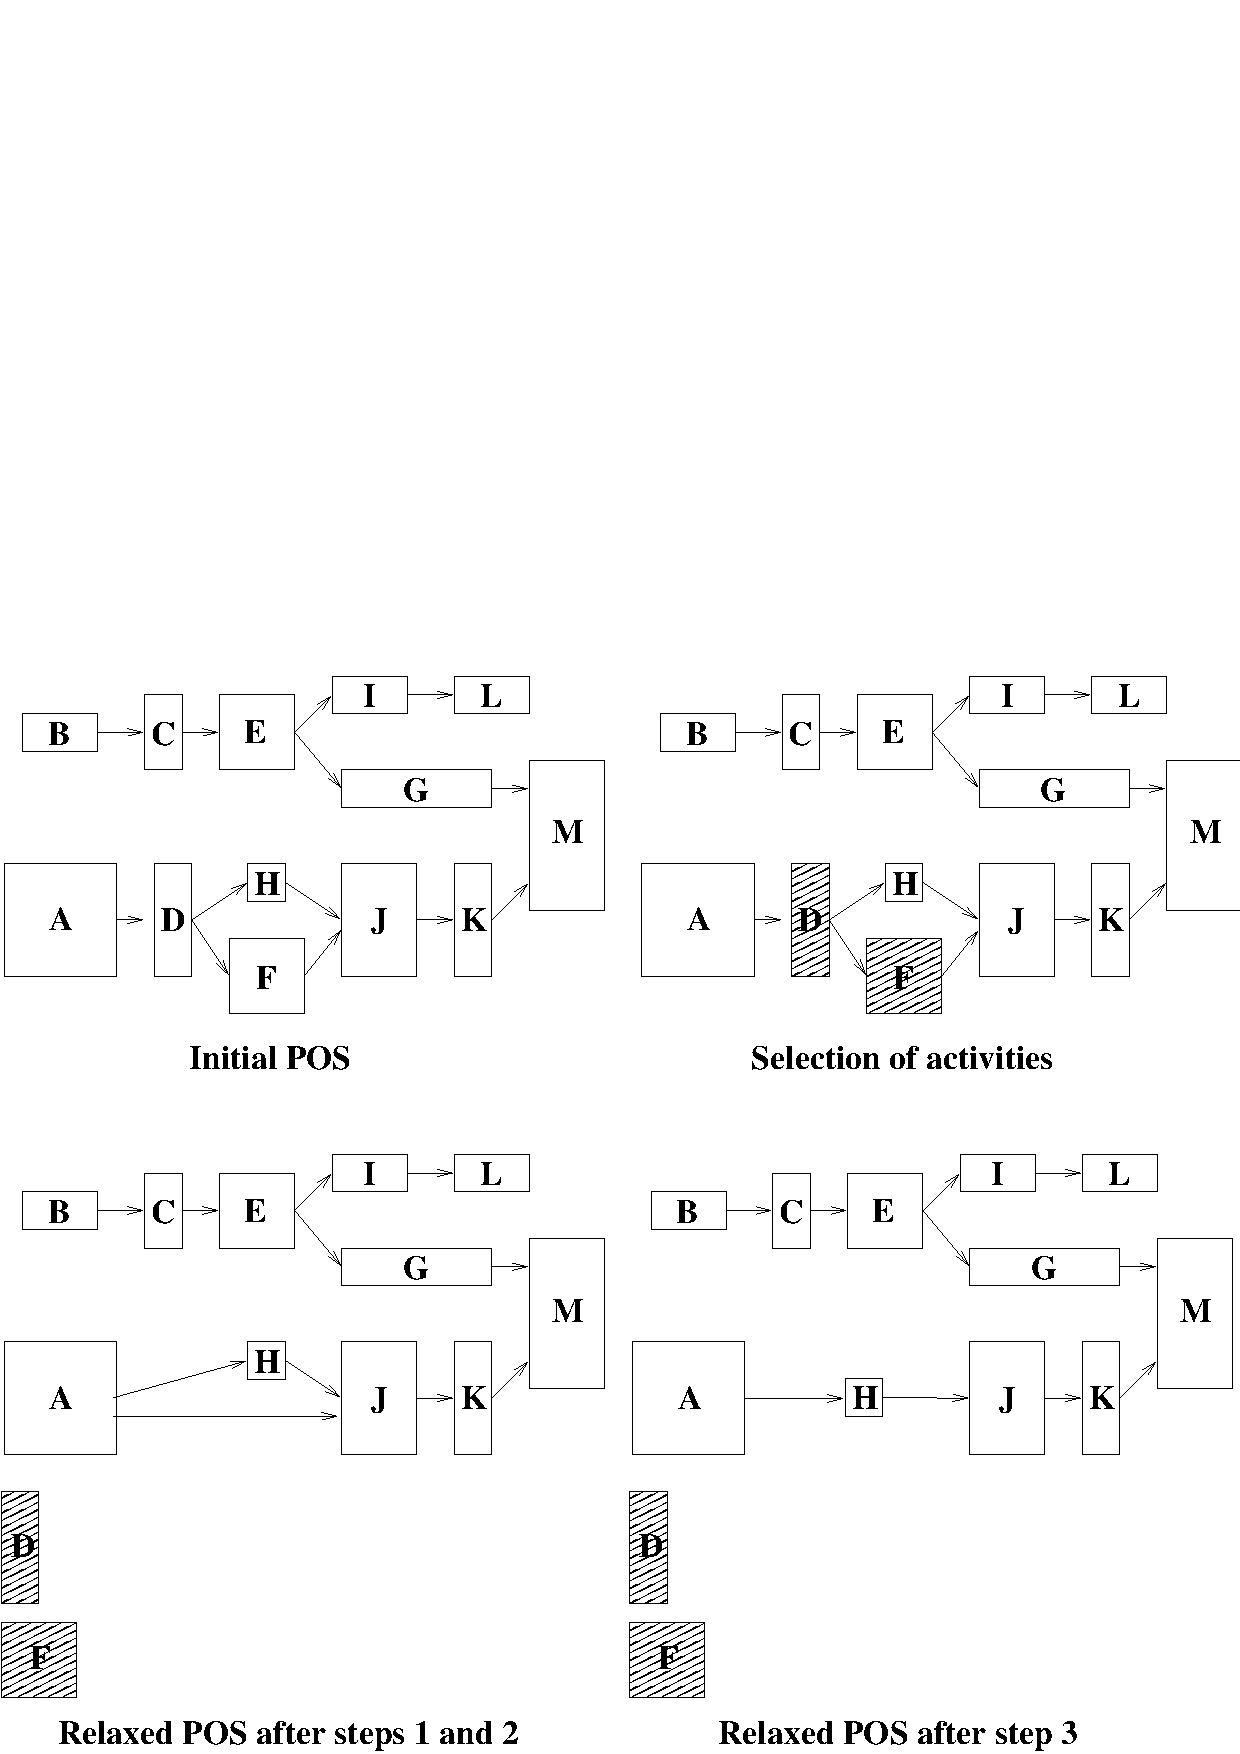
\includegraphics[width=8cm]{figures/pos-relax.pdf}
	\caption{Computing a \emph{Relaxed POS}}
	\label{fig:computingRelaxedPOS}
\end{figure}

The temporal constraints of the obtained relaxed POS are then taken as
new start point for the next iteration of the LNS. In our study, to
build the set of selected activities $S$ we choose them randomly with
a probability $\alpha$ which is a parameter of the algorithm. It means
that in average, $m=\alpha\ |\calA|$.

This large neighborhood search has been implemented by using
the LNS framework available in {\sc ILOG Scheduler} 6.1~\cite{scheduler61}.

\subsection{Iterative Improvement}

The iterative improvement procedure we use is described in Algorithm
\ref{alg:alg2}. The name of the algorithm - $STRand$ - stands for {\bf
S}et{\bf T}imes + {\bf Rand}om relaxation. We used the {\em SetTimes}
procedure with three parameters:
\begin{itemize}
\item parameter $\gamma$ that specifies the maximum allowed number of
backtracks (expressed in percentage of the number of activities) for one execution of the procedure,
\item a flag $f\!c \in \{ first, cont\}$ that tells whether the search must stop at
the first solution found or continue search trying to minimize the makespan until the maximum number of
backtracks $\gamma$ is reached (or an optimal solution found), and
\item an upper bound $ub$ on the makespan.
\end{itemize}

The parameter $\gamma$ allows to control the {\em SetTimes} procedure from a simple descent ($\gamma=0$ no backtracks allowed) to a complete search tree ($\gamma=\infty$).

The input parameters of $STRand$ are: the problem $P$ to solve, the
probability $\alpha$ to relax a given activity in the $RandomRelax$
procedure ($0<\alpha\leq1$), the improvement step $\beta$, the maximum
number of backtracks $\gamma$, the flag $f\!c$, and a global time
limit $t$.

\begin{algorithm}
	\caption{Iterative Improvement Algorithm}
	\label{alg:alg2}
	\begin{algorithmic}[1]
  \Procedure{STRand}{$P$,$\alpha$,$\beta$,$\gamma$,$f\!c$,$t$}
		\State $R := P$
		\State $m^* := \infty$ \Comment{$m^*$: Best makespan so far}
		\State $ub := \infty$ \Comment{$ub$: Upper bound for SetTimes}
		\While{$time < t$}
			\State $s := \mathrm{SetTimes}(R,\gamma,f\!c,ub)$ \label{reoptimize}
			\If{($makespan(s) < best$)}
				\State $s^* := s$      \Comment{$s^*$: Best schedule so far}
				\State $m^* := makespan(s)$ 
			  \State $ub := (1+\beta) m^*$
			\EndIf
			\State $R := \mathrm{POSRelax}(P,s)$
			\State $R := \mathrm{RandomRelax}(R,P,\alpha)$
		\EndWhile
		\State \textbf{return} $s^*$
		\EndProcedure
	\end{algorithmic}
\end{algorithm}

\subsection{Constraint Propagation}

When re-optimizing a relaxed solution $R$ at line \ref{reoptimize},
the number of precedence relations may be large as $R$ contains a
subset of the temporal constraints generated when converting the
fixed-time schedule to a \emph{POS}. To efficiently propagate these
temporal constraints, we have implemented two algorithms:
\begin{itemize}
	\item A topological sort on the direct acyclic graph of
	temporal constraint is used to compute the initial time bounds
	of the activities. The complexity of this algorithms is
	$O(n+p)$ where $n$ is the number of activities and $p$ the
	number of temporal constraints. This algorithm is run only
	once at each iteration.
	\item The algorithm described in \cite{Michel2003} to
	incrementally maintain the longest paths in direct acyclic
	graphs is used to incrementally compute the time bounds of
	activities. The complexity of this algorithm is in
	$O(\left\|\delta\right\| \log\left\|\delta\right\|)$ where
	$\left\|\delta\right\|$ is a measure of the change in the
	graph since the previous propagation. This algorithm is activated
	after each decision taken during the search procedure.
\end{itemize}

This temporal propagation was implemented as a global constraint in
the CP framework of {\sc ILOG Solver}~\cite{solver61} and {\sc ILOG Scheduler}~\cite{scheduler61}. The capacity of
resources is propagated using the {\em timetable} constraint of {\sc
ILOG Scheduler} \cite{lepape-94}.

\section{Computational Results}\label{SCompRes}

In this section, we report the computational results of the algorithm
described in the previous section.

\subsection{Benchmarks}

The benchmarks we used are the standard benchmarks from
~\cite{Nuijten94}. These benchmarks are derived from job shop
scheduling problems by introducing a certain number of duplicates for
each job and increasing the capacity of the resources
accordingly. The benchmarks are classified in 5 groups:

\begin{itemize}
	\item \textbf{Set A} : Lawrence LA01-LA10 duplicated and triplicated.
	\item \textbf{Set B} : Lawrence LA11-LA20 duplicated and triplicated.
	\item \textbf{Set C} : Lawrence LA21-LA30 duplicated and triplicated.
	\item \textbf{Set D} : Lawrence LA31-LA40 duplicated and triplicated.
	\item \textbf{Set MT} : MT06, MT10, and MT20 duplicated and triplicated.
\end{itemize}

Because of the way these instances are constructed, upper bounds on
the optimal makespan can be derived from the corresponding job shop
scheduling instances. Incidently, the results of
~\cite{Michel2004,Cesta2000,NuijtenAarts96} have shown that these
upper bounds are not so easy to find as the algorithms used are not
aware of the underlying structure of the instances. Notice also that
the instances by construction contain equivalent solutions. In our
study, as in previous ones, no constraint has been used to break those
symmetries.

In terms of size, with these different sets we have quite a large
spectrum ranging from 50 to 900 activities and from 5 to 15
resources. Sets A, B, and MT consist of small to medium size
instances whereas sets C and D consist of medium to large size
instances. 


\subsection{Preparing Time Equivalent Tests}
% was \subsection{Computing Average Running Times}

To conduct fair comparisons both between our approach and previously
reported approaches as well as between different parameter settings for our
approach we aim to do time equivalent tests. To do so we determined
maximum running times for each instance in the following way. First,
we applied a search procedure that is comparable in complexity to the
ones used by~\cite{Cesta2000,Michel2004} by allowing no backtracks
during search ($\gamma=0$), i.e., the search procedure {\em SetTimes} either
returns a solution obtained without any backtracking or stops as soon
as a backtrack occurs. To allow a better comparison to
\cite{Michel2004} we use the same stop criterion they used, i.e., the
algorithm is stopped if for a certain number of iterations the
solution was not improved. We set this maximum number of so called
{\em stable iterations} to $1000$. The other parameters are as follows~: $\alpha=0.2$, 
and $\beta=0$. For each instance we then do 10
runs and take the average CPU time as maximum running time that we
will use throughout our experiments for that instance.

The machine used for the computational study is a Pentium 4 at 2.8
Ghz. Average results reported are always computed over 10 runs unless
specified otherwise.

%WN. I did not include the table giving the running times per set of
%instances. These averages are thus averages over a whole set, times
%differ per used machine, and what's more people can redo the
%experiments we did. This is more than what normally can be said.


\subsection{Results Summary}

We found the best performance for our approach when choosing the
following values for the different parameters: $\alpha=0.2$,
$\beta=0$, $\gamma=0.15$, and $f\!c=cont$. Running time for each instance was
limited to the maximum running time computed in the previous section.

Table~\ref{tab:QualityComparison} reports average deviation
(in percentage) from the upper bounds ({\em UB}) reported
in~\cite{NuijtenAarts96} and used in the evaluation
in~\cite{Cesta2000} and in~\cite{Michel2004}.

As can be observed, our results are on average significantly better
both in terms of quality and robustness than the ones published in
\cite{Cesta2000} and
\cite{Michel2004}. Table~\ref{tab:QualityComparison} summarizes prior
results of algorithm \emph{$IFlat_5$} (iterative flattening procedure
with 5 random restarts as in \cite{Cesta2000}) and algorithm
\emph{IFlatIRelax 4(20)} (relax probability of 20\% and a number of
relaxations of 4 as in \cite{Michel2004}) with respectively 1000, 5000
and 10000 iterations. The column \emph{STRand 1000} reports the 
results obtained when computing average running times.

\begin{table}[htbp]
  \centering
	\scriptsize
	\begin{tabular}{c|c|c|c|c|c|c}
	  Set& $IFlat_5$ & \multicolumn{3}{c|}{IFlatIRelax 4(20)} & STRand & STRand\\
	  & & 1000 & 5000 & 10000 & 1000 & 0.2/0/0.15/cont \\
	  \hline
	  A   & 7.76 & 1.63 & 1.07 & 0.90& 0.14 & \textbf{-0.13} \\
	  B   & 7.10 & 1.04 & 0.47 & 0.24& -0.59 & \textbf{-1.10} \\
	  C   & 13.03 & - & 4.2    & -   & 1.18 &  \textbf{-0.16} \\
	  D   & 11.92 & - & 2.4    & -   & 1.11 &  \textbf{0.22} \\
	  MT  & - & 4.76 & 3.41    & 3.12& 1.30 &  \textbf{0.55} \\
	  \hline		
	  Total &  &     & 2.13 &        & 0.59 & \textbf{-0.23} \\
	  \hline
	\end{tabular}
	\caption{Results summary of $IFlat_5$, $IFlatIRelax$ and $STRand$}
	\label{tab:QualityComparison}
\end{table}

On average, $STRand(\alpha=0.2, \beta=0, \gamma=0.15, f\!c=cont)$ is
within -1.10\% and 0.55\% of \emph{UB}. Furthermore, we have obtained 
new upper bounds on 33 instances out of 86. 

For detailed results, see Section {\em Detailed Results} below.

\subsection{Impact of the Relaxation Probability}

To study the influence of the different parameters we did a series of
tests. We firstly studied the influence of varying the relaxation
probability $\alpha$. Table~\ref{tab:ImpactOfRelaxtionProbability}
reports average deviation in percentage from {\em UB} when $\alpha$ is
varying between $0.1$ and $0.3$. Running time for each instance is
limited to the maximum running time computed previously. The other
parameters are as follows: $\beta=0$, $\gamma=0.15$, and $f\!c=cont$.

\begin{table}[htbp]
	\centering
		\begin{tabular}{c|c|c|c|c|c|c|c|c}
			Set & $0.1$ & $0.15$ & $0.2$ & $0.25$ & $0.3$ \\
			\hline
			A     &  0.09 & -0.09 & \textbf{-0.13} & -0.12 & \textbf{-0.13} \\
			B     & -0.57 & -0.87 & -1.10 & \textbf{-1.26} & -1.25 \\
			C     & -0.27 &	\textbf{-0.41} &	 -0.16 &  0.32 &  0.58 \\
			D     &  0.52 &  0.25 &  \textbf{0.22} &  0.33 &  0.58 \\
			MT    &  1.15 &  0.76 &  0.55 &  \textbf{0.39} &  0.43 \\
			\hline
			Total &  0.03 &	-0.21 &	\textbf{-0.23} &	-0.14 &	 0.01 \\
			\hline
		\end{tabular}
	\caption{Impact of the Relaxation Probability $\alpha$ on $STRand(\alpha, \beta=0, \gamma=0.15, f\!c=cont)$}
	\label{tab:ImpactOfRelaxtionProbability}
\end{table}

Overall the best results are obtained with $\alpha=0.2$ although the quality 
obtained with $\alpha=0.15$ is very closed. It gives the best results on 2 sets 
while $\alpha=0.15$ works better for set C and $\alpha=0.25$ works better for 
set B and set MT.


\subsection{Impact of the Improvement Step}

Table~\ref{tab:ImpactOfImprovementStep} reports the average deviation
in percentage from \emph{UB} when the improvement step $\beta$ is varying from
$-\epsilon$ (enforce to find a solution strictly better than the best
solution so far) to $\infty$ (no enforcement at all). Running time for
each instance is limited to the maximum running time computed
previously. The other parameters are as follows: $\alpha=0.2$,
$\gamma=0.15$, and $f\!c=cont$.

\begin{table}[htbp]
	\centering
		\begin{tabular}{c|c|c|c|c}
			Set & $-\epsilon$ & $0$ & $0.01$ & $\infty$ \\
			\hline
			A	    &  0.23 & \textbf{-0.13} &  0.16 & 1.15 \\
			B	    & -0.37 & \textbf{-1.10} & -0.53 & 0.77 \\
			C	    &  0.76 &  \textbf{-0.16} &  3.54 & 5.50 \\
			D	    &  0.92 &  \textbf{0.22} &  2.31 & 3.21 \\
			MT    &  1.58 &  \textbf{0.55} &  1.03 & 3.90 \\
			\hline
			Total &  0.47 & \textbf{-0.23} &  1.35 & 2.74 \\
			\hline
		\end{tabular}
	\caption{Impact of the Improvement Step $\beta$ on
	$STRand(\alpha=0.2, \beta, \gamma=0.15, f\!c=cont)$}
	\label{tab:ImpactOfImprovementStep}
\end{table}

For positive improvement steps, increasing the value leads to
increasing the average deviation and thus decreasing the quality. The
best quality is obtained with a null improvement step, that is when
the search procedure is enforced to find a solution better or equal to
the previous one. Results obtained when applying $-\epsilon$ as
improvement step are not as good. With $-\epsilon$ we observe that the
first iterations decrease the cost effectively, but then the search is
often trapped in a local optimum. 

%We plan to study dynamic adaption
%schemes of $\alpha$ as used in \cite{NuijtenLePape98} to escape from
%these local minima, which in turn may change the influence of $\beta$.

\subsection{Impact of the Maximum Number of Backtracks}

Table~\ref{tab:ImpactOfNumberOfBacktracks} reports the average
deviation in percentage from \emph{UB} when the maximum number of
allowed backtracks $\gamma$ is varying from 0\% to 20\% with the number of activities. 
Running time for each instance is limited to the maximum running time computed
previously. The other parameters are as follows: $\alpha=0.2$,
$\beta=0$, and $f\!c=cont$.

\begin{table}[htbp]
	\centering
		\begin{tabular}{c|c|c|c|c|c|c}
			Set & $0$ & $0.05$ & $0.10$ & $0.15$ & $0.20$ & $0.50$ \\
			\hline
			A     &  0.42 & \textbf{-0.16} & -0.15 & -0.13 & \textbf{-0.16} & -0.13 \\
			B     &	-0.67 & -1.06 & -1.07 & \textbf{-1.10} & -1.09 & -1.06 \\
			C     &  0.87 &  -0.14 &  \textbf{-0.17} &  -0.16 &  -0.06 & -0.01 \\
			D     &  0.91 &  0.24 &  0.25 &  0.22 &  \textbf{0.18} & 0.28 \\
			MT    &  1.21 &  \textbf{0.38} &  0.64 &  0.55 &  0.52 & 0.66 \\
			\hline
			Total &  0.44 & \textbf{-0.23} & -0.22 & \textbf{-0.23} & -0.22 & -0.17 \\
			\hline
		\end{tabular}
	\caption{Impact of the Number of Backtracks $\gamma$ on $STRand(\alpha=0.2, \beta=0, \gamma, f\!c=cont)$}
	\label{tab:ImpactOfNumberOfBacktracks}
\end{table}

Overall, for $\gamma$ varying between 5\% and 20\%, there is no much difference in quality. Increasing $\gamma$ further than 20\% leads to increasing the average deviation and thus decreasing the quality.

\subsection{Impact of the Search Method}

Table~\ref{tab:ImpactOfSearchMethod} compares the average deviation in
percentage from \emph{UB} when continuing search at each iteration
until all allowed backtracks are exhausted with the one obtained when
stopping search at the first solution found. Running time for each instance
is limited to the maximum running time computed previously. The other
parameters are as follows: $\alpha=0.2$, $\beta=0$, and $\gamma=0.15$.

\begin{table}[htbp]
	\centering
		\begin{tabular}{c|c|c}
			Set & $first$ & $cont$\\
			\hline
			A     & \textbf{-0.13} & \textbf{-0.13} \\
			B	    & -0.98 & \textbf{-1.10} \\
			C     &  0.09 &  \textbf{-0.16} \\
			D     &  0.38 &  \textbf{0.22} \\
			MT    &  0.60 &  \textbf{0.55} \\
			\hline
			Total & -0.11 & \textbf{-0.23} \\
			\hline
		\end{tabular}
	\caption{Impact of the Search Method on $STRand(\alpha=0.2, \beta=0, \gamma=0.15, f\!c=first/cont)$}
	\label{tab:ImpactOfSearchMethod}
\end{table}

When continuing search obviously more time is taken at each iteration:
the search returns the best solution found using the limited amount of
backtracks instead of returning the first solution found. As the time
is limited, this implies less iterations. As can be observed
continuing search leads to improved quality on all sets of instances.

\subsection{Detailed Results}
\label{DetailedResults}

Tables~\ref{tab:ResultsSetA}, \ref{tab:ResultsSetB},
\ref{tab:ResultsSetC}, \ref{tab:ResultsSetD} and
\ref{tab:ResultsSetMT} display in the second column the lower bounds
reported in \cite{NuijtenAarts96} including some recent improvements
described in \cite{Laborie2005} followed by the upper
bounds found by~\cite{NuijtenAarts96} or derived from the
corresponding job shop scheduling instance. If these two values are
equal, only one number is given. The third column reports
the upper bounds found by~\cite{Michel2004}. The following three
columns report the best upper bounds, the average upper bounds and the
average running time obtained when performing 1000 stable
iterations. The following two columns report the best upper bounds and the average
upper bounds obtained with $STRand$ when using the following parameters:
$\alpha=0.2$, $\beta=0$, $\gamma=0.15$, and $f\!c=cont$. Running time for
each instance is limited to the maximum running time computed
previously. Best and average upper bounds are computed over 10 runs. The
last column reports the best overall upper bound obtained with
$STRand$ during this study. Results are in bold when a new upper bound
is reported. Note that this last column indeed reports the best upper
bounds found during all the tests we did during this computational
study, not just the best of the two parameter settings reported on in
this section.

\begin{table}[htbp]
	\centering
	\tiny
		\begin{tabular}{c|c|c||c|c|c||c|c||c}
			\hline
			Instance & LB/UB & MvH & 
			\multicolumn{3}{c||}{Avg Running Times} &
			\multicolumn{2}{c||}{0.2/0/0.15/cont} &  
			Best  \\
			&&& best & avg & time & best & avg & \\
			\hline
			la01d & 666     & -   & 666 & 666 &  1 & 666 & 666 & 666 \\
			la01t & 666     & -   & 666 & 666 &  1 & 666 & 666 & 666 \\
			la02d & 655     & -   & 655 & 659 & 18 & 655 & 657 & 655 \\
			la02t & 655     & -   & 655 & 659 & 39 & 655 & 656 & 655 \\
			la03d & 593/597 & -   & 597 & 604 & 15 & 596 & 603 & \textbf{593} \\
			la03t & 590/597 & -   & 596 & 600 & 35 & 595 & 599 & \textbf{592} \\
			la04d & 572/590 & 577 & 578 & 607 & 13 & 576 & 578 & \textbf{576} \\
			la04t & 570/590 & 584 & 579 & 608 & 27 & 574 & 577 & \textbf{573} \\
			la05d & 593     & -   & 593 & 593 &  1 & 593 & 593 & 593 \\
			la05t & 593     & -   & 593 & 593 &  1 & 593 & 593 & 593 \\
			la06d & 926     & -   & 926 & 926 &  1 & 926 & 926 & 926 \\
			la06t & 926     & -   & 926 & 926 &  1 & 926 & 926 & 926 \\
			la07d & 890     & -   & 890 & 890 &  4 & 890 & 890 & 890 \\
			la07t & 890     & -   & 890 & 891 & 35 & 890 & 890 & 890 \\
			la08d & 863     & -   & 863 & 863 &  2 & 863 & 863 & 863 \\
			la08t & 863     & -   & 863 & 863 & 20 & 863 & 863 & 863 \\
			la09d & 951     & -   & 951 & 951 &  1 & 951 & 951 & 951 \\
			la09t & 951     & -   & 951 & 951 &  1 & 951 & 951 & 951 \\
			la10d & 958     & -   & 958 & 958 &  1 & 958 & 958 & 958 \\
			la10t & 958     & -   & 958 & 958 &  1 & 958 & 958 & 958 \\
		\end{tabular}
	\caption{Detailed Results on Set A}
	\label{tab:ResultsSetA}
\end{table}


On set $A$, new upper bounds for all 4 open instances have been found.
All results reported in~\cite{Michel2004} are improved ({\tt la04d} and
{\tt la04t}). Instance {\tt la03d} is now closed.

\begin{table}[htbp]
	\centering
	\tiny
		\begin{tabular}{c|c|c||c|c|c||c|c||c}
			\hline
			Instance & LB/UB & MvH & 
			\multicolumn{3}{c||}{Avg Running Times} &
			\multicolumn{2}{c||}{0.2/0/100/cont } &  
			Best  \\
			&&& best & avg & time & best & avg & \\
			\hline
			la11d 	&	1222	&	 - 	&	1222	&	1222	&	1	&	1222	&	1222	&	1222	\\
			la11t 	&	1222	&	 - 	&	1222	&	1222	&	1	&	1222	&	1222	&	1222	\\
			la12d 	&	1039	&	 - 	&	1039	&	1039	&	2	&	1039	&	1039	&	1039	\\
			la12t 	&	1039	&	 - 	&	1039	&	1039	&	34	&	1039	&	1039	&	1039	\\
			la13d 	&	1150	&	 - 	&	1150	&	1150	&	1	&	1150	&	1150	&	1150	\\
			la13t 	&	1150	&	 - 	&	1150	&	1150	&	11	&	1150	&	1150	&	1150	\\
			la14d 	&	1292	&	 - 	&	1292	&	1292	&	1	&	1292	&	1292	&	1292	\\
			la14t 	&	1292	&	 - 	&	1292	&	1292	&	1	&	1292	&	1292	&	1292	\\
			la15d 	&	1207	&	 - 	&	1207	&	1207	&	9	&	1207	&	1207	&	1207	\\
			la15t 	&	1207	&	 - 	&	1207	&	1207	&	47	&	1207	&	1207	&	1207	\\
			la16d 	&	 892/935 	&	929	&	931	&	940	&	46	&	925	&	935	&	\textbf{925}	\\
			la16t 	&	 887/935 	&	927	&	922	&	935	&	92	&	921	&	929	&	\textbf{918}	\\
			la17d 	&	 754/765 	&	756	&	756	&	761	&	44	&	755	&	760	&	\textbf{755}	\\
			la17t 	&	 753/765 	&	761	&	764	&	765	&	78	&	755	&	762	&	\textbf{755}	\\
			la18d 	&	 803/844 	&	818	&	815	&	829	&	46	&	811	&	823	&	\textbf{811}	\\
			la18t 	&	 783/844 	&	813	&	816	&	821	&	99	&	808	&	816	&	\textbf{808}	\\
			la19d 	&	 756/840 	&	803	&	816	&	824	&	43	&	804	&	814	&	\textbf{795}	\\
			la19t 	&	 740/840 	&	801	&	808	&	813	&	97	&	792	&	798	&	\textbf{787}	\\
			la20d 	&	 849/902 	&	864	&	872	&	908	&	47	&	859	&	875	&	\textbf{859}	\\
			la20t 	&	 842/902 	&	863	&	872	&	876	&	101	&	862	&	871	&	\textbf{854}	\\
		\end{tabular}
	\caption{Detailed Results on Set B}
	\label{tab:ResultsSetB}
\end{table}


On set $B$, new upper bounds have been found for all 10 open
instances. All improve results reported in~\cite{Michel2004}.

\begin{table}[htbp]
	\centering
	\tiny
		\begin{tabular}{c|c|c||c|c|c||c|c||c}
			\hline
			Instance & LB/ UB & MvH & 
			\multicolumn{3}{c||}{Avg Running Times} &
			\multicolumn{2}{c||}{0.2/0/100/cont } &  
			Best  \\
			&&& best & avg & time & best & avg & \\
			\hline
			la21d 	&	 1017/1046 	&	 - 	&	1038	&	1046	&	203	&	1037	&	1042	&	\textbf{1034}	\\
			la21t 	&	 1012/1046 	&	 - 	&	1064	&	1073	&	479	&	1039	&	1042	&	\textbf{1027}	\\
			la22d 	&	 913/927 	&	 - 	&	939	&	948	&	94	&	926	&	936	&	\textbf{926}	\\
			la22t 	&	 913/927 	&	 - 	&	936	&	943	&	295	&	929	&	934	&	928	\\
			la23d 	&	1032	&	 - 	&	1032	&	1032	&	34	&	1032	&	1032	&	1032	\\
			la23t 	&	1032	&	 - 	&	1032	&	1033	&	142	&	1032	&	1032	&	1032	\\
			la24d 	&	 885/935 	&	932	&	911	&	927	&	168	&	903	&	913	&	\textbf{903}	\\
			la24t 	&	 884/935 	&	929	&	924	&	935	&	414	&	904	&	907	&	\textbf{898}	\\
			la25d 	&	 907/977 	&	 - 	&	958	&	970	&	140	&	954	&	960	&	\textbf{952}	\\
			la25t 	&	 903/977 	&	965	&	954	&	965	&	502	&	945	&	952	&	\textbf{945}	\\
			la26d 	&	1218	&	 - 	&	1218	&	1219	&	234	&	1218	&	1219	&	1218	\\
			la26t 	&	1218	&	 - 	&	1220	&	1225	&	615	&	1218	&	1219	&	1218	\\
			la27d 	&	1235	&	 - 	&	1244	&	1255	&	394	&	1237	&	1245	&	1235	\\
			la27t 	&	1235	&	 - 	&	1259	&	1273	&	790	&	1242	&	1249	&	1241	\\
			la28d 	&	1216	&	 - 	&	1234	&	1258	&	265	&	1222	&	1235	&	1216	\\
			la28t 	&	1216	&	 - 	&	1256	&	1270	&	457	&	1239	&	1252	&	1216	\\
			la29d 	&	 1117/1152 	&	 - &	1150	&	1168	&	581 &	1137	&	1147	&	{\bf 1131}	\\
			la29t 	&	 1116/1152 	&	 - &	1199	&	1212	&	743	&	1144	&	1153	&	{\bf 1130}	\\
			la30d 	&	1355	&	 - 	&	1355	&	1359	&	129	&	1355	&	1355	&	1355	\\
			la30t 	&	1355	&	 - 	&	1355	&	1358	&	363	&	1355	&	1357	&	1355	\\
		\end{tabular}
	\caption{Detailed Results on Set C}
	\label{tab:ResultsSetC}
\end{table}


On set $C$, 9 new upper bounds upon 10 open instances have been found
({\tt la21d}, {\tt la21t}, {\tt la22d}, {\tt la24d}, {\tt la24t}, {\tt
  la25d}, {\tt la25t}, {\tt la29d}, and {\tt la29t}). All 3 upper bounds reported in~\cite{Michel2004} are improved.

\begin{table}[htbp]
	\centering
	\tiny
		\begin{tabular}{c|c|c||c|c|c||c|c||c}
			\hline
			Instance & LB/UB & MvH & 
			\multicolumn{3}{c||}{Avg Running Times} &
			\multicolumn{2}{c||}{0.2/0/100/cont } &  
			Best  \\
			&&& best & avg & time & best & avg & \\
			\hline
			la31d 	&	1784	&	 - 	&	1784	&	1784	&	55	&	1784	&	1786	&	1784	\\
			la31t 	&	1784	&	 - 	&	1784	&	1784	&	211	&	1784	&	1784	&	1784	\\
			la32d 	&	1850	&	 - 	&	1850	&	1850	&	1	&	1850	&	1850	&	1850	\\
			la32t 	&	1850	&	 - 	&	1850	&	1850	&	2	&	1850	&	1850	&	1850	\\
			la33d 	&	1719	&	 - 	&	1719	&	1719	&	65	&	1719	&	1719	&	1719	\\
			la33t 	&	1719	&	 - 	&	1719	&	1719	&	464	&	1719	&	1719	&	1719	\\
			la34d 	&	1721	&	 - 	&	1721	&	1721	&	199	&	1721	&	1722	&	1721	\\
			la34t 	&	1721	&	 - 	&	1721	&	1722	&	695	&	1721	&	1721	&	1721	\\
			la35d 	&	1888	&	 - 	&	1888	&	1892	&	240	&	1888	&	1891	&	1888	\\
			la35t 	&	1888	&	 - 	&	1888	&	1894	&	877	&	1888	&	1890	&	1888	\\
			la36d 	&	 1229/1268 	&	 - 	&	1255	&	1266	&	251	&	1251	&	1260	&	\textbf{1250}	\\
			la36t 	&	 1227/1268 	&	 - 	&	1259	&	1265	&	636	&	1247	&	1256	&	\textbf{1247}	\\
			la37d 	&	 1378/1397 	&	 - 	&	1444	&	1458	&	243	&	1418	&	1432	&	1416	\\
			la37t 	&	 1370/1397 	&	 - 	&	1445	&	1456	&	676	&	1428	&	1439	&	1419	\\
			la38d 	&	 1092/1196 	&	1185	&	1200	&	1230	&	431	&	1179	&	1199	&	\textbf{1175}	\\
			la38t 	&	 1087/1196 	&	1195	&	1197	&	1224	&	1278	&	1173	&	1189	&	\textbf{1168}	\\
			la39d 	&	 1221/1233 	&	 - 	&	1242	&	1255	&	297	&	1228	&	1231	&	\textbf{1226}	\\
			la39t 	&	 1221/1233 	&	 - 	&	1252	&	1257	&	731	&	1227	&	1237	&	\textbf{1226}	\\
			la40d 	&	 1180/1222 	&	 - 	&	1241	&	1245	&	340	&	1214	&	1223	&	\textbf{1205}	\\
			la40t 	&	 1176/1222 	&	 - 	&	1245	&	1253	&	786	&	1219	&	1225	&	\textbf{1206}	\\
		\end{tabular}
	\caption{Detailed Results on Set D}
	\label{tab:ResultsSetD}
\end{table}

On set $D$, 8 new upper bounds upon 10 open instances have been
found ({\tt la36d}, {\tt la36t}, {\tt la38d}, {\tt la38t}, {\tt
  la39d}, {\tt la39t}, {\tt la40d}, and {\tt la40t}) and the 2 upper bounds reported in~\cite{Michel2004} are improved.

\begin{table}[htbp]
	\centering
	\tiny
		\begin{tabular}{c|c|c||c|c|c||c|c||c}
			\hline
			Instance & LB/UB & MvH & 
			\multicolumn{3}{c||}{Avg Running Times} &
			\multicolumn{2}{c||}{0.2/0/100/cont } &  
			Best  \\
			&&& best & avg & time & best& avg & \\
			\hline
			mt06d 	&	55	&	 - 	&	56	&	56	&	5	&	55	&	56	&	55	\\
			mt06t 	&	55	&	 - 	&	55	&	56	&	12	&	55	&	55	&	55	\\
			mt10d 	&	 837/930 	&	913	&	899	&	913	&	63	&	901	&	917	&	\textbf{891}	\\
			mt10t 	&	 828/930 	&	912	&	889	&	897	&	177	&	882	&	890	&	\textbf{879}	\\
			mt20d 	&	1165	&	1186	&	1209	&	1223	&	62	&	1183	&	1209	&	1182	\\
			mt20t 	&	1165	&	1205	&	1206	&	1220	&	157	&	1189	&	1211	&	1179	\\
		\end{tabular}
	\caption{Detailed Results on Set MT}
	\label{tab:ResultsSetMT}
\end{table}

On set $MT$, new upper bounds have been found for the two open
instances ({\tt mt10d} and {\tt mt10t}). On {\tt mt20d} and {\tt
mt20t}, $STRand$ also finds a better solution than ever reported
before but still does not reach the upper bound derived from the
corresponding job shop scheduling instances.

Overall, we improved 33 upper bounds upon 36 open instances. For the 3
remaining open instances ({\tt la22t}, {\tt la37d}, and {\tt la37t})
we found solutions with a makespan that was not yet reported before,
although we did not yet find a schedule with a makespan better than or
equal to the upper bound derived from the corresponding job shop
scheduling instance. This also goes for 3 closed instances ({\tt
la27t}, {\tt mt20d}, and {\tt mt20t}). On all other instances, the
optimal schedule has been systematically found. Note thus that for
many of these instances it is the first time a schedule was found with
a makespan equal to the makespan that can be derived from the
corresponding job shop scheduling instances.


\section{Conclusion}\label{SConclusion}

In this paper we described a generic approach to solve cumulative
scheduling problems based on randomized large neighborhood search. We
presented a way to calculate a partial-order schedule from a fixed
start time schedule, which is a crucial step in the generalization to
cumulative scheduling from earlier randomized LNS work for disjunctive
scheduling. We applied and
tested the approach on the Cumulative Job Shop Scheduling Problem. The
empirical performance analysis we performed using a well-known set of
benchmark instances showed that our approach obtains the best known
performance reported to date on the CJSSP. New upper bounds have been
found on 33 out of 36 open instances and among them one instance is now closed. 
Furthermore, our approach proves to be very robust on the complete set of test instances.
As for future work, we plan to study how our approach
competes on other types of problems such as the Resource Constrained
Project Scheduling Problem. Another direction we plan to study is how
this approach can be extended, on one hand to other types of resources
such as state resources and discrete reservoirs, and on the other hand
to other types of objectives such as earliness/tardiness costs and
resource allocation costs. Flexibility of the generated POS is clearly 
a key factor for the approach. We plan to compare the flexibility of 
our POS generation procedure with the one of \cite{Policella2004} and 
work on improving this flexibility by exploiting interactions between resources.

\bibliography{mybibliography}
\bibliographystyle{plain}

\end{document}






Removed because trivial.
\begin{algorithm}
	\caption{Random Selection}
	\label{alg:alg1}
	\begin{algorithmic}[1]
  \Procedure{RandomSelection}{$\alpha$}
		\State $S := \emptyset$
		\ForAll{$a_i \in \calA$}
			\If{$\mathrm{RANDOM(0,1)} \leq \alpha$}
				\State $S := S \cup \left\{a_i\right\}$
			\EndIf
		\EndFor
		\EndProcedure
	\end{algorithmic}
\end{algorithm}




%Removed to improve clarity of presentation.
%In set A, instances vary from (10, 5) to (45,5). In set B,
%instances vary from (40, 5) to (60,5) and from (20, 10) to (30,
%10). In sets C, instances vary from (20, 10 to (60, 10). In set C,
%instances vary from (60, 10) to (90, 10) and from (30, 15) to (45,
%15).

%It is often difficult to compare one's results to previously published
%results for several reasons: use of different languages (i.e. Java or
%C++), different machines (CPUs, memory, bus), some encapsulate
%algorithms in a generic framework or library while others implement
%specific algorithms entirely dedicated to solve a specific type of
%problem. Furthermore, published results do not always provide detailed
%information on each instance... 


Removed:
Table~\ref{tab:ResultsWith1000Iterations} reports the average running
times. The following
parameters have been used: relaxation probability $\alpha=0.2$,
improvement step $\beta=0$ (solution must be better or equal to the
previous one) and maximum number of backtracks $\gamma=0$.

\begin{table}[htbp]
	\centering
		\begin{tabular}{c|c|c|c}
			Set& Best dev. & Average dev. & Time \\
			\hline
			A &  0.19 &  0.52 & 15 \\
			B & -1.00 & -0.63 & 59 \\
			C &  0.90 &  1.58 & 498 \\
			D &  0.55 &  1.05 & 561 \\
			MT & 0.69 &  1.50 & 111 \\
			\hline
		\end{tabular}
	\caption{Results of STRand with 1000 Iterations}
	\label{tab:ResultsWith1000Iterations}
\end{table}


Removed because not useful anymore:
Notice that the results obtained with a $\gamma=0$ are
slightly different from the ones reported in
Table~\ref{tab:ResultsWith1000Iterations}. This is due, for each
instance, to the use of the average time limit computed with $1000$
stable iterations over all the seeds. This time limit is here the same
for each seed whereas on Table \ref{tab:ResultsWith1000Iterations},
the time is varying from seed to seed depending on the actual time it
takes to perform $1000$ stable iterations.



\begin{table}[htbp]
	\centering
		\begin{tabular}{c|c|c|c|c|c}
			Set& IFlatIRelax 4(20) & STRand & STRand\\
			& 5000 & 1000 & 0.2/0/100/cont \\
			\hline
			A  & 1.07 &  0.52 & \textbf{-0.12} \\
			B  & 0.47 & -0.63 & \textbf{-0.91} \\
			C  & 4.2  &  1.58 &  \textbf{0.33} \\
			D  & 2.4  &  1.05 &  \textbf{0.42} \\
			MT & 3.41 &  1.50 &  \textbf{0.47} \\
			\hline
			Total & 2.13 & 0.69 & \textbf{-0.03} \\
			\hline		
		\end{tabular}
	\caption{Results summary}
	\label{tab:ResultsSummary}
\end{table}

